\documentclass[a4paper, 10pt]{article}
\usepackage[utf8]{inputenc}
\usepackage{graphicx}
\usepackage[T1]{fontenc}
\usepackage[french]{babel}
\usepackage{listings}
\usepackage{amssymb}
\usepackage{amsmath}
\usepackage{fullpage}
\usepackage{url}
\usepackage{authblk}
\usepackage{hyperref}

\usepackage[final]{pdfpages}

\begin{document}

\title{Parallel Minimum Spanning Tree using MPI}
\author{BETHUNE Louis}
\date{December 2017}

\maketitle

\section{Implementation choices}  
  
According to me, minimum spanning tree is not an algorithm we can easily parallelize. In fact, sequential algorithms are already very effective : $\mathcal{O}(E\ln(E))$. So I supposed that the parallelization was made mainly as answer to memory issues.  
  
I implemented the sequential algorithms in the way that they're fast on sparse graphs, and the parallel ones in the way they're fast on dense graphs.  

\subsection{Sequential Kruskal}

For this algorithm I used the union-find structure to test if there is cycles. I used both union by rank and path compression optimizations to obtain the best complexity of $\mathcal{O}(n\alpha(n))$ where $\alpha(n)$ is the inverse Ackermann function.  
  
The edges are sorted using \textbf{qsort}, the quick sort of standard C library.  
  
\subsection{Sequential Prim}

For this algorithm the border (the array $D$) is not explicitly maintained. In fact, I used a heap to store the border. Thanks to this I can ask the closest vertex in $\mathcal{O}(1)$ at each step of the iteration. 
  
Moreover, at each iteration, the lazy heap doesn't contain more data than the number of edges of the border. For this reason, this algorithm is very effective on sparse graphs. However it may lead to bad performances on dense ones.  

\subsection{Parallel Prim}

My implementation is very close from the pseudo-code provided. There's no heap used. So we expect the execution time of the algorithm to only depend of the number of vertices, regardless that the graph is sparse or not. So this algorithm is a good candidate for dense graphs.  
  
However on sparsest ones it doesn't benefit of the parallelization at all (for exemple, a line of vertices).  
  
The vertex $z$ associated to each $y$ in the array $D$ is stored, and updated in $\mathcal{O}(1)$. Thanks to this optimization, the inner loop of the algorithm is executed in $\mathcal{O}(p + \frac{n}{p})$ (first term corresponds to the work of processor $0$, and second one to the others).  
  
\newpage
\subsection{Parallel Kruskal}  
  
The algorithm proposed in both versions of the problem statement is very confusing, because there is a lot of possible interpretations. Because of this, I choose to implement a version maybe hardest than the one demanded. It's not something taken on internet (or something else) but a new version the algorithm I didn't see elsewhere.
  
\subsubsection{The algorithm}
  
At the beginning, each processors holds $\frac{n}{p}$ vertices and their edges. Let's call this set $\mathbb{F}_{k,i}$ : the forest of size $2^{k-1}\times\frac{n}{p}-1$ hold by processor $i$, with $k = 0$.  
  
Then, if $i+1$ is odd then the processor $i+1$ sends its forest to processor $i$, and the edges between their two forests.  
Processor $i-1$ merges the two forest (using the edges) to form $\mathbb{F}_{1,i}$.  
  
In the general case, at step $k$, processor $i+2^k$ sends forest $\mathbb{F}_{k,i+2^k}$ to processor $i$. Moreover the processors between $i+1$ and $i+2^k$ send their edges between $\mathbb{F}_{k,i+2^k}$ and $\mathbb{F}_{k,i}$. Processor $i$ merges these edges to form $\mathbb{F}_{k+1,i}$.  
  
You can see illustration of this on the following picture. Initial forests $\mathbb{F}_{0,i}$ are the dark blue squares; Edges between two initials forests are in yellow. After merge operation, $\mathbb{F}_{1,i}$ is hold by processors of even rank : it corresponds to empty red squares. Between two $\mathbb{F}_{1,i}$ the edges are the dark khaki squares. In general, empty squares are the forests, and filled squares are the edges between forests. Some arrows are drawn to show from what and to what the data are send.  
  
\begin{center}
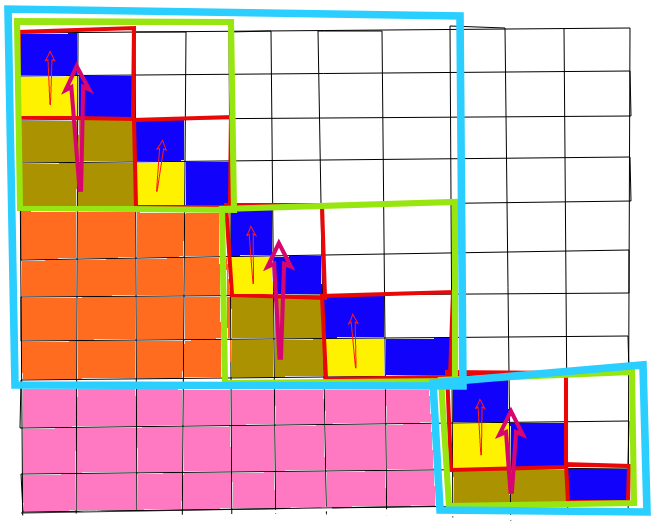
\includegraphics[scale=0.28]{final.png}  
\end{center}
  
A given processor is a \textbf{receiver} until it sends its first forest. After that, it's not a receiver anymore. It becomes a \textbf{sender}. It will send edges between two other forests for the rest of the algorithm. A given processor is receiver for as many steps than the number of $0$ before the first $1$ in the binary expansion of its rank. For this reason the main loop of the algorithm uses \textit{bitwise operations}.  
  
A sender sends its forest \textbf{exactly once}. But it will send edges as many times it has $1$ in the binary expansion of its rank. The processor computes the spanning forest of these edges before sending them. Note that these edges corresponds to a bipartite graph. Thanks to this, the sends are very costless (even in dense graph). This is a good property with environment with small bandwith.  
  
The receiver performs the merge operation. As the receiver receives $2^k$ messages, each of size at most $(2^k+1)\times\frac{n}{p}-1$, it must merge them. But the edges from these messages are already sorted. So to avoid a new sorting operation of cost $\mathcal{O}(E\ln{E})$ we perform a merge operation between $2^k$ sorted lists in $\mathcal{O}(2^k\times E)$.   
  
This algorithm is pretty well balanced compared to the others. Instead of perform a big kruskal on a local forest, and then a big send with this forest, it alternates Kruskal operations with sends operations, on sets with size that grows exponentially. So, at each step, \textbf{atmost the half of the processors doesn't work}, half of them perform a send (with the associated Kruskal), and an exponentially decreasing numbers of processors perform a merge between sets of small sizes.  
  
The algorithm stop when $2^k > P$ so when $k = \log P$. The number of steps is logarithmic in the input size when $P = O(n)$. So this algorithm is very good when we have few thousand of cores. This may seem irrealistic but it's common on a supercalculator, or when we have few dozen of GPU (that have been shown to be very successful in high performance computing). Unfortunately, when we have $P = O(\sqrt{N})$ it doesn't achieve so much.  
  
Thanks to Leonard Assouline for its help to formally prove that this algorithm was correct.  
  
\subsubsection{Implementation}  
  
A merge of sorted list needs the output list to be different from the input lists (there is no efficient in-place merge). So a naive implementation of $2^k$ will demand $2^k$ more copies of the array. I improve this by swapping the pointers (instead of the arrays) of the input and output lists.  
  
Each array is allocated with the right size (up to byte precisely). So the memory consumption is low (excepting the size of the adjency matrix).  
  
\section{Results}
My hardware consists in an Intel(R) Core(TM) i3-4010U CPU @ 1.70GHz, with 4 Go RAM.  
  
The points on the graphic are computed using a mean on 10 executions to decrease errors dues to execution in a stochastic environement (personal computer).  
  
I modified the squeleton to send the computation time on stderr instead of stdout. It was easier for me to separate the list of edges and the computation.
  
Squares correspond to kruskal algorithm, and diamonds to prim algorithm.   
\subsection{Sequential algorithms}   
\subsubsection{Sparse graphs}
Test are done on graphs family with constant average degree $d$. There is one curv for each algorithm used and each $d$.  
  
In x-axis there is the number of vertices of the graph, and in y-axis the execution time in seconds.  
  
Blue curvs corresponds to average degree of $25$, green to average degree of $10$ and red to average degree of $5$.  
  
\begin{center}
\includegraphics[scale=0.6]{sparseSeq.png}
\end{center} 
  
We see that Kruskal always perform better in practice on sparse graphs (as expected). But we also see that the execution time grows quadratically. This is a serious issue, because these alorithms are very effective (linearithmic) on adjency lists, but the adjency matrix representation is the bottleneck of all of this. This is not a factor I can improve because it's my input.  
\subsection{Dense graphs}  
On dense graph, in x-axis we found the number of edges, and as usual the y-axis count the execution time in seconds. The maximum numbers of edges of graph with $n$ nodes is $\frac{n(n-1)}{2}$. Here we take half of this quantity. So the average degree is $\frac{n}{2}$. Unfortunately I was unable to generate a graph with more than $25000000$ edges, due to memory issues.  
  
I made several other tests with a smallest average degree (but keeping the graph dense anyway). But I don't show them here because it appears that the execution time seems totally independant of the number of nodes (points corresponding to the same amount of edges, regardless the number of nodes, were supperposed). Only the total number of edges matters, and this is already cover by the following curvs.  
  
\begin{center}
\includegraphics[scale=0.6]{denseSeq.png}
\end{center} 
\subsection{Parallel Algorithms}
Evaluate performance of parallel algorithms on a sequential machine (my personnal computer with two physical cores... ) is very hard. I used smpi to test different parameters, like the number of cores, the latency, the bandwith...  
  
I wrote a file named gen\_clique.py that generate platforms and hostfile for a clique topology. This kind of topology is very rare in practice (except, maybe, when we use processors like Intel Xeon Phi that contains few dozen of cores). But I wanted to test my algorithms in idyllic situation.  
  
I used data from \url{https://milkyway.cs.rpi.edu/milkyway/cpu_list.php} to choose the speed power of each host. Unfortunately, smpi doesn't provide realistic computation time. I think smpi is made to see how good a algorithm scales (by testing different parameters), but should not be used in the way to obtain exact computation time.  
  
First, I fixed the host speed to 8.8GF, the latency to 10us, and the bandwith to 100Gbps. These values seemed realistic.  
  
\subsubsection{Sparse}  
  
Prim is the red curb, kruskal the blue one. In ordered there is the execution time, and in abscissa the number of cores. Because the smpirun is \textbf{very slow} (it takes more than one hour to make benchmarks) I only test $1$, $2$, $3$, $4$, $8$, $16$, $32$, and $64$ cores. I used the graph with $10000$ nodes and $250000$ edges.  
  
Here I choose a logarithmic scale because on a linear scale it was impossible to see something.  
  
\begin{center}
\includegraphics[scale=0.6]{sparsePar.png}  
\end{center}
  
What can we notice ? Kruskal is improved by the parallelization, except when the number of cores is bigger than $32$. Why ? Because bigger the number of cores is, bigger the number of send/receive is. When each processor does too few work (because there is too much processors), most of the time is spent in send/receive instead of doing computations.  
  
However, the result for Prim is awful. For the same reasons : there is one send/receive per processor for each new edge added to the tree. This amount of communications is so huge that, without a very good bandwith and a very low latency, it's not worth it.  
  
\subsubsection{Dense}  
  
Here I used the graph with $9000$ nodes and $20247750$ edges.  
  
\begin{center}
\includegraphics[scale=0.6]{densePar.png}  
\end{center}
  
Concerning Kruskal, the results are very impressive. The speedup is quasi-linear. I would like to make test with more and more processors (let's say $512$ or $1024$ but we need $P \leq \sqrt{N}$).  
  
As usual, Prim doesn't perform well at all, for the same reasons than previously. Moreover due to a too high computation time I didn't get any result for Prim parallel running with 64 cores.  
  
\subsubsection{Future work}  
  
We see that Prim requires a big numbers of small communications, so Prim is very sensitive to latency but not too much to bandwith.  
  
However Kruskal does only a few amount of communications, but these communications are huge. So Kruskal is verys sensitive to bandwith, and not too much to latency.  
  
Verify this demands a lot of experiments and I didn't make them.    
  
\section{Conclusion}  
  
Prim algorithm doesn't scale very well. Kruskal is amazingly effective, both in sequential and parallel, because it can use the cache cleverly. Parallization is useful only on dense graphs, else it doesn't bring so much.  
  
Adjency matrix is a data structure that leads to serious bottleneck on sparse graph, making the benchs useless.  
\end{document}
  